% Carsten: 
% This chapter should come much earlier.
% Perhaps not everything, but at least DNV GL should be introduced and their motivations should be stated before even starting with the state-of-the-art reviews. 
% That means that section 5.1 of chapter 5 should be an own chapter between chapters 1 and 2. It would provide the fundamental reasons for making your thesis.
% In that new chapter, you should describe the approval workflow as it is today: papers is sent back and forth, models are made and updated on both sides, 
% annotations are disconnected from designs. And the vision: a share digital design where designer and reviewer can interact, perhaps even meet in a cooperative mode, 
% but without loosing the accountability that comes from today’s paper trail. This story of DNV GL’s vision is important - you must come back to it at the start of chapter 6.
% 
% It should also preferably be longer: more about what DNV GL is, what classification comprises, focus onto ships in this thesis. Where in the long line of 
% classification-related tasks does your thesis fit?
% The rest of 5 is in the right place. However, the current chapter 4 should really come after you have stated your requirement into this chapter.

\section{The Roles of Classification Societies}
A classification society provides classification, statutory services and assistance to the maritime industry based on its accumulated knowledge of fields like
maritime, engineering, construction and technology~\citep{Hormann2006}.
The International Association of Classification Societies (IACS) defines a classification society as an organization which
publishes its own classification rules and technical requirements in relation to the design, construction or survey of ships. 
The organization should have capacity to apply, maintain and update these rules and requirements with own resources on a regular basis, and should 
be impartial, meaning that it should not be controller by ship-owners, shipbuilders or be otherwise commercially engaged in the manufacture, 
equipping, repair or operation of ships.
In addition the classification society should verify compliance with these rules and requirements during construction and periodically during a classed
ship's service life. 

% Kanskje droppe dette avsnittet?
Classification societies dates back to the second half of the 18th century, where marine insurers developed a system for independent technical assessment of the ships
presented to them for insurance cover. These insurers were based out of Lloyd's Coffee House, a popular establishment for sailors, merchants and shipowners, and led to
the establishment of the insurance market Lloyd's of London, Lloyd's Register and several related shipping and insurance businesses~\cite{Marcus1975}.
This also led to a committee being formed in London in 1760 being the first recorded classification society committee~\citep{Hormann2006}. 
At this time, various aspect of a ship, such as its hull and equipment, were assigned "grades" for their condition, ranging between G, M and B (good, middling or bad), 
or simply 1, 2 and 3. As the classification profession evolved, these different classifications were mostly replaced by a more discrete classification system, meaning
a ship either meets the relevant class society's rules or it does not. 

This classification serves as a certification process where the candidate 
has to fulfill a number of requirements in order to "pass" the classification process. 
\citet{Hormann2006} describes the objective of ship classification as verifying "the structural strength and integrity of essential parts of the ship’s hull 
and its appendages, and the reliability and function of the propulsion and steering systems, power generation and those other features and auxiliary systems 
which have been built into the ship in order to maintain essential services on board. Classification Societies aim to achieve this objective through the development 
and application of their own Rules and by verifying compliance with international and/or national statutory regulations on behalf of flag Administrations"
This is a thorough and continuous evaluation process that has several phases~\citep{Hormann2006}. These phases include:

\begin{itemize}
	\item A technical review of the design plans and related documents for a new vessel to verify compliance with the applicable rules and requirements.
	\item Attendance at the construction site of the vessel by a classification society surveyor to verify that the vessel is 
		  constructed in accordance with the approved design plans and classification rules.
	\item Attendance at relevant production facilities that provide key components such as the steel, engine, generators and castings to verify that the components conforms to
		  the rules and requirements.
	\item Attendance at the sea trials and other trials relating to the vessel and its equipment.
	\item Upon satisfactory completion of the above, the builder’s/shipowner’s request for the issuance of a class certificate will be considered by the 
		  relevant classification society and, if deemed satisfactory, the assignment of class may be approved and a certificate of classification issued.
	\item Once in service, the owner must submit the vessel to a clearly specified program of periodical surveys, carried out on board the vessel, 
		  to verify that the ship continues to meet the relevant rules and requirements for its class.
\end{itemize}

\begin{figure}%[h!] %[H]
	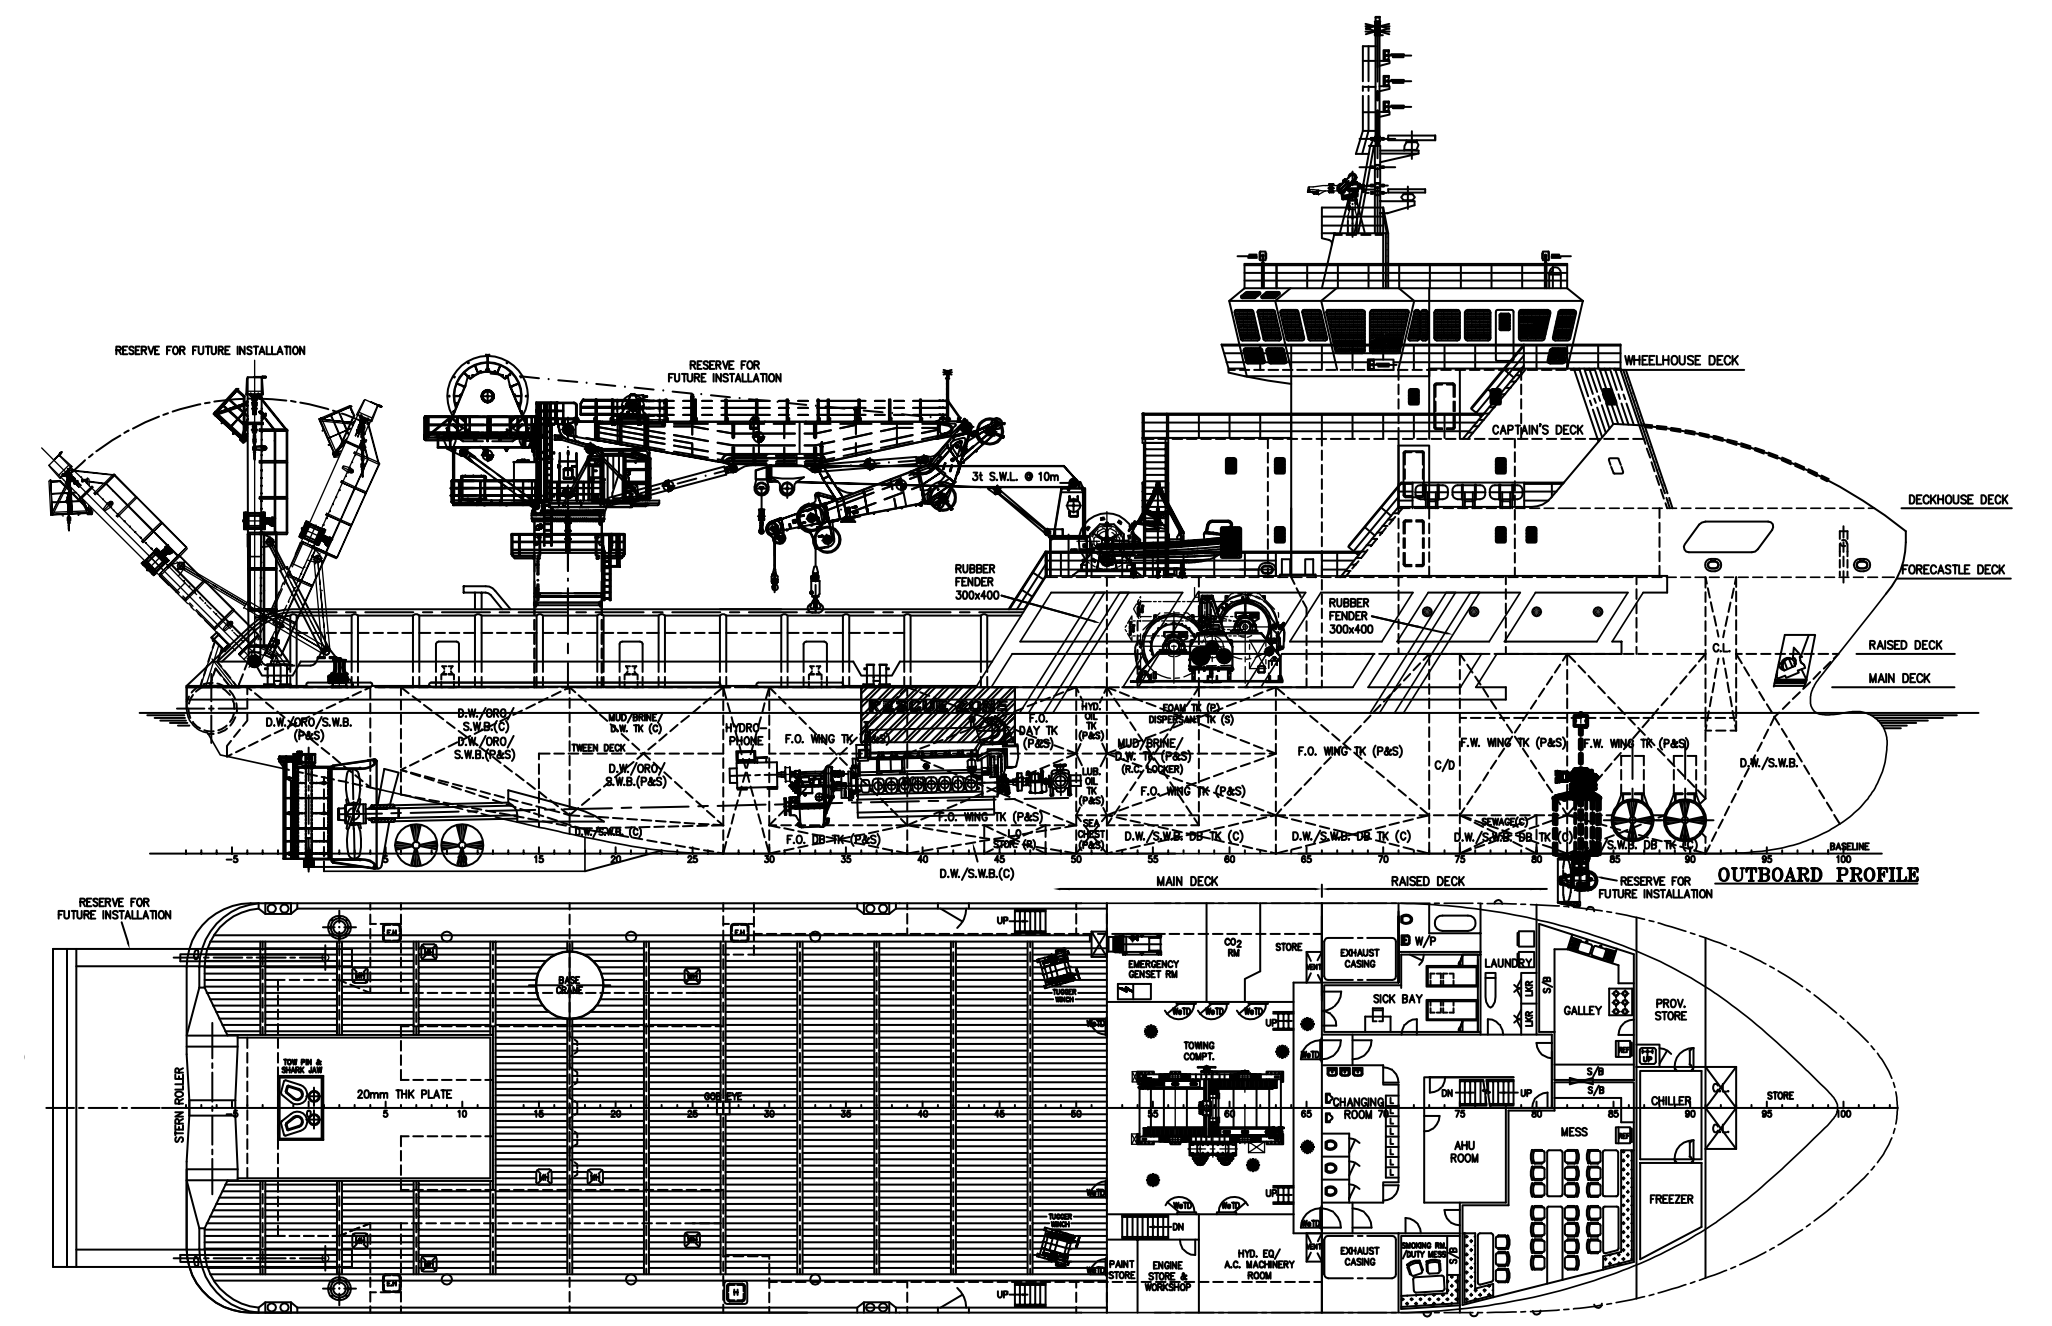
\includegraphics[width=\linewidth]{pictures/ship_design_sketch.png}
	\caption[A typical paper based design sketch]{A typical paper based design sketch~\cite{MarinoConsult}}
	\label{fig:ship_design_sketch}
\end{figure} 

The first phase, i.e the technical review of the design plans, is of special interest to this thesis as it is one that stands to gain a lot from 
new ways of utilizing computer technology. The use of customized high quality software in this phase can potentially improve the entire work flow and enable useful 
features such as e.g.~ keeping a history of decision, changes and discussions, in addition to organize the information in an intuitive manner. 
As we will see in the next sections, this phase already commonly makes use of high fidelity 3D models, but often in a much more narrow fashion than 
what could be possible. 

\section{DNV GL's Digital Vision}
DNV GL is the result of a merger, taking place in 2013, between two leading classification societies, Det Norske Veritas (Norwegian) and Germanischer Lloyd (Germany),
and is the world's largest classification society with about 15,000 employees and 350 offices operating in more than 100 countries. 
They provide services for more than 13 000 vessels and mobile offshore units, which represents a global market share of 21\%~\citep{TO:DNVGL}
It is the world's largest technical consultancy to onshore and offshore wind, wave, tidal, and solar industries, as well as the global oil \& gas industry 
-- 65\% of the world’s offshore pipelines are designed and installed to DNV GL technical standards~\citep{MTN:DNVGL}. 

As a classification society, DNV GL operates in all the phases outlines above and, as mentioned in chapter~\vref{chapter:introduction}, they are 
currently investigating the idea of a virtual reality application for technical design reviews. 
Currently their technical design review process can be summarized by the following steps: 

\begin{enumerate}
	\item The designer sends the model to DNV GL for evaluation.
	\item One or several "approval engineer" from DNV GL inspects the model noting down (usually on a document) aspects that doesn't meet DNV GL requirements.
	\item The designer receives the remarks and has to make the necessary changes to the model to continue to process towards getting the classification.
	\item This process is repeated until the design is approved.
\end{enumerate}

This process usually results in a lot of papers being sent back and forth, and because of a lack of application support the process can, according to one DNV GL employee,
feel very disconnected and "ad hoc". 

Although digital 3D models usually are utilized in this phase, the work flow is reportedly still mostly based on design document and drawings.  
It is said that the model is usually just a reference, and is static (i.e receives no changes) throughout the process. After the model is "completed", and DNV GL starts
its design review process, most (if not all) comments, annotations and discussions are handled separate from the model (e.g.~through emails, phone calls)
and is highly paper-based. This might in part because of the existing computer-aided design (CAD) software solution and in part because of the established practices.

DNV GL is thus looking into the possibilities of digitalizing this process more, and making it more interactive and efficient by 
conduct virtual design review meetings in the 3D models. Here the designer and reviewer could interact, 
survey the model together, and annotate it instead of model-printouts (on paper). This should also be possible 
without loosing the accountability that comes from today’s paper trail. It is thus not necessarily the 3D models themselves that 
need to evolve, but rather the application that interfaces with them and what functionality they allow for.  

As the sense of scale is important in a 3D model review, virtual reality technology is deemed promising as it gives a unique sense of scale
and a depth, which is hard to match by regular "2D screens". 
DNV GL is also interested in alternate interaction methods, as mouse and keyboard can have some limitation when working in a 3D environment~\citep{Rautaray2015}. 
Gesture Recognition Technology has been of special interest as this can potentially offer unique approaches to working with 3D models.

\begin{figure}%[h!] %[H]
	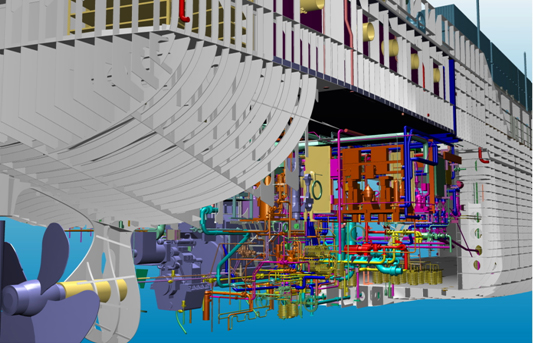
\includegraphics[width=\linewidth]{pictures/ship_cad.jpg}
	\caption[A ship model created using conventional CAD software.]{A ship model created using conventional Computer-aided Design (CAD) software.~\cite{IMO}}
	\label{fig:ship_cad}
\end{figure} 


\section{Initial Design Ideas}
The core functionality of such an application should be to navigate the 3D model and "annotate" it (i.e creating and placing remarks tied to a the model), 
primarily by using the advantages of virtual reality and gesture recognition technology. 
The users should also be able to create "sessions" that enable several users to be virtually present 
in the same instance of the 3D model, and to interact with it using gestures. During these sessions a user should then be able to create annotations, 
which can be interacted with (e.g.~edited or deleted) and are tied to the 3D model and the session. 

Actions done during the 3D model session (such as annotating an object) should continuously be stored in a database. 
If a user wants to re-enter the session at a later time, this database is read, and the actions done in previous sessions are loaded into the model.
By utilizing a database 
in this way the model files themselves can also remain unedited throughout a session, as opposed to saving annotations into the model files itself, 
which could be more inefficient and create model versioning issues. 
Another upside with utilizing a database is that it enables exposure of the actions done in the sessions to other platforms, such as web applications. 
This can enable annotation and comments done on the 3D model to become "issues" or "remarks" in more traditional collaboration tools such as Atlassian's Jira or Confluence.

% Write more on initial design ideas?
To approach these design ideas this thesis will first review the fields of virtual reality technology and gesture recognition technology, before revisiting the design in light
of these reviews. The design is concretized and scoped in chapter~\vref{chapter:design}, where we select the focus and core functionality and write these as 
"user stories" (i.e informal, natural language descriptions of features, commonly used in software projects). Here we will also go more into the design issues that has to be
addressed before the implementation starts, and review our technology choices.  




% INCLUDE USE CASES HERE?


% A major part of DNV GL's work is evaluation and quality assurance of a client's product (e.g.~a ship) , 
% where a DNV GL "Approval Engineer" conducts a design review of the client's model of the proposed product. 